%%%%%%%%%%%%%%%%%%%%%%%%%%%%%%%%%%%%%%%%%%%%%%%%%%%%%%%
%                 File: OSAstyle.tex                  %
%                     VERSION: 3.1                    %
%                Date: May 28  2004                   %
%                                                     %
%    LaTeX template file for use with OSA journals    %
%         JOSA A, JOSA B, Applied Optics, and         %
%                   Optics Letters                    %
%                                                     %
%   This file requires the substyle file osajnl.rtx,  %
%       running under REVTeX 4.0 and LaTeX 2e,        %
%                           or                        %
%   the style file osajnl.sty, running under LaTeX 2e %
%                                                     %
%       USE THE FOLLOWING REVTEX 4.0 OPTIONS:         %
%  \documentclass[osajnl,preprint,showpacs]{revtex4}  %
%                                                     %
%         USE THE FOLLOWING LaTeX OPTIONS:            %
%           \documentclass[12pt]{article}             %
%           \usepackage{osajnl}                       %
%                                                     %
%                                                     %
%      NOTE: LaTeX 2.09 IS NO LONGER SUPPORTED        %
%                                                     %
%      (C) 2004 The Optical Society of America        %
%                                                     %
%%%%%%%%%%%%%%%%%%%%%%%%%%%%%%%%%%%%%%%%%%%%%%%%%%%%%%%

% \documentclass[12pt,osajnl,preprint,showpacs]{revtex4}  %% REVTeX 4.0

%%%%%%%%%%%%%%%%%%%%%%%%%%%%%%%%%%%%%%%%%%%%%%%%%%%%%%%%%%%%%%%%
%% Delete any REVTEX output files before running in LaTeX mode
%%%%%%%%%%%%%%%%%%%%%%%%%%%%%%%%%%%%%%%%%%%%%%%%%%%%%%%%%%%%%%%%%

\documentclass[letterpaper,12pt]{article}   %% LaTeX 2e (preferred)
\usepackage{osajnl} %% do not use with REVTeX4
\usepackage[draft]{hyperref} %% optional

\begin{document}

\title{Preparing a manuscript
for the Optical Society of America journals JOSA A, JOSA B, \\
\textit{Applied Optics}, and \textit{Optics Letters}}

\author{Scott Dineen, Alexine Moore, and Joseph Richardson}
%% for REVTeX4, each author name can be set in a separate \author{} field

\address{Optical Society of America, 2010 Massachusetts Avenue, NW, \\
Washington, D.C. 20036} %\affiliation will also work

\email{alias@osa.org}

\begin{abstract}A style guide and template for JOSA A, JOSA B,
\textit{Applied Optics}, and \textit{Optics Letters} manuscripts
is provided with a focus on use of \LaTeXe\ and REV\TeX{}4. A
basic template, \texttt{osatemp.tex}, is also included in this
distribution. Additional detailed instructions for manuscript
preparation and submission are available on the home page for each
OSA journal; see \mbox{\href{http://www.opticsinfobase.org}{http://www.opticsinfobase.org}}. \\
\end{abstract}

\ocis{000.0000, 999.9999.}% REPLACE WITH CORRECT OCIS CODES FOR YOUR ARTICLE
                          % NOTE: \ocis{} IS ALIASED TO \pacs{} BUT MUST
                          % FORMAT THE TERMS CORRECTLY FOR EACH JOURNAL

\maketitle %% null function with osajnl.sty

\section{Introduction}
Adherence to the specifications listed in this guide is essential
for efficient review and publication. For additional guidelines on OSA style see the 
\textit{OSA Print Journal Style Guide} on individual journal pages on  
\mbox{\href{http://www.opticsinfobase.org}{http://www.opticsinfobase.org}}.


\section{Page Layout and Length}
Paper size for electronic submissions should be U.S. Letter, 8.5
in. $\times$ 11 in. (approximately 21.5 cm $\times$ 28 cm). 
Interline spacing has been changed from 2 to 1.2 to help save space. Recommended page length for manuscripts varies with each journal. 

Note that \textit{Optics Letters} (OL) has a strict limit of
three printed, i.e.---final typeset---pages. Mandatory page
charges or higher publication fees apply to papers above each
journal's length limit.
\section{Software}
\subsection{Package Files}
The package file \texttt{osajnl.sty} calls up
\texttt{overcite.sty} (citations), \texttt{graphicx.sty} (replaces \texttt{graphics.sty}), and \texttt{geometry.sty} (page layout). Additional
package files should be used when needed (e.g.,
\texttt{hyperref.sty}, as used in this document). Use of
nonstandard or custom package files is discouraged; however, if
such files are essential, they should be included with the
manuscript submission.

\subsection{\LaTeX{} and REV\TeX} Most versions of \LaTeXe{}
available as freeware, shareware, or commercially will run the OSA
\LaTeX{} files correctly. Authors who choose to use REV\TeX{}
should obtain the latest REV\TeX{}4 package from the American
Physical Society (\url{http://www.aps.org}) or from the
Comprehensive \TeX{} Archive Network (CTAN;
\href{http://www.ctan.org}{http://www.ctan.org}) and become familiar with REV\TeX{}4's
special features. Note that certain packages, such as
\verb+natbib+, that may be required for proper operation of
REV\TeX{} are not necessarily included in the standard REV\TeX{}4
distribution and should be obtained separately.

\subsection{Compressing Files for Submission}
Authors submitting \LaTeX{} or REV\TeX{} files should create a
tarred, gzipped archive of their \texttt{.tex} file and all
figures (which should be in EPS digital format). All files must be
referenced at the root level (e.g., file {\tt OT00000F1.eps}, not
\verb+\EPSDIR\OT00000F1.eps+).  Authors who submit a \LaTeX{} or REV\TeX{} file
with no figures may submit an ASCII text file without compression
or archiving. {\bf Note that submission of \TeX-generated
PostScript files is not allowed}.

\subsection{REV\TeX{} and \LaTeX{} Support}
The subfile \texttt{osajnl.rtx} is REV\TeX{}4 compliant. REV\TeX{} and
\LaTeX{} commands for title, author, address, and e-mail are
supported. The \verb+\pacs{}+ command has been made an alias of
\verb+\ocis{}+; \verb+\affiliation{}+, an alias of
\verb+\address{}+. With little effort, a manuscript prepared in
the REV\TeX{}4 substyle for another society's journal can be
converted to OSA style. The style commands that may be used at the
start of a manuscript for submission to JOSA A, JOSA B,
\textit{Applied Optics}, and \textit{Optics Letters} are
\begin{verbatim}
   \documentclass[osajnl,preprint,showpacs]{revtex4} %%REVTeX 4.0
    
    or
   
   \documentclass[12pt]{article} %%LaTeX 2e
   \usepackage{osajnl}
\end{verbatim}

Note that \LaTeX{} packages for \href{http://www.opticsexpress.org}{\textit{Optics Express}} and the \href{http://www.osa-jon.org}{\textit{Journal of Optical Networking}} should be obtained separately.


\section{Main Text}
\subsection{Typographical Style}
Margins and type size will be set by the OSA REV\TeX{} or \LaTeX{}
commands for title, author names and addresses, abstract,
references, captions, and so on. Use of custom macros and style
files is discouraged.



\subsection{Title}
Only the first letter in the title is
capitalized, except for proper names and abbreviations (note that
abbreviations should be spelled out in most cases in manuscript
and section titles). Place the title within the braces of the
\verb+\title{}+ command.


\subsection{Author Names}
Author names should be given in full and consistent form to
facilitate indexing. Every effort should be made to keep author
names consistent from one paper to the next as they appear within
OSA publications.  For REV\TeX{} set each author name off with a
separate \verb+\author{}+ command above the appropriate
affiliation. REV\TeX{} will add commas and the word ``and.'' For
\LaTeX, author names should be grouped together, as appropriate,
with proper punctuation.

\subsection{Author Affiliations}
Affiliations should follow the format division, organization, and
address---and complete postal information should be given.
Abbreviations should not be used. Place each affiliation within
the braces of the \verb+\affiliation{}+ command to achieve the
correct format.

\bigskip

For REV\TeX:
\begin{verbatim}
\author{Alessandra Gatti}
\author{Luigi Alberto A. Lugiato}
\affiliation{Instituto Nazional di Fisica per la Materia,
Dipartmento Di Fisica, \\ Via  Celoria 16, 20133 Milano, Italy}
\end{verbatim}

\bigskip

For \LaTeX:
\begin{verbatim}
\author{Gian-Luca Oppo and Richard Martin}
\affiliation{Department of Physics, University of Strathclyde, \\
Rottenrow 107, Glasgow G4 ONG, Scotland}
\end{verbatim}

\subsection{Abstract} Authors should place the abstract between
the following commands to achieve the correct format: \
\verb+\begin{abstract}+ and \verb+\end{abstract}+. The abstract
should be limited to approximately 100 words. It should be an
explicit summary of the paper that states the problem, the methods
used, and the major results and conclusions. If the research of
another author is referenced in the abstract, complete information
(e.g., journal, volume number, first page, year) must be
given in the abstract itself.

\subsection{OCIS Subject Classification} Optics Classification and
Indexing Scheme (OCIS) subject classifications should be placed at
the end of the abstract with the \verb+\ocis{}+ command. OCIS
codes can be found at \href{http://www.osa.org/pubs/authors/ocis/}{http://www.osa.org/pubs/authors/ocis/}.

\subsection{Mathematical and Scientific Notation}
\subsubsection{Displayed Equations} Equations should be centered.
Equation numbers should appear at the right-hand margin, in
parentheses:
\begin{equation}
H = \frac{1}{2m}(p_x^2 + p_y^2) + \frac{1}{2} M{\Omega}^2
     (x^2 + y^2) + \omega (xp_y - yp_x).
\end{equation}

All equations should be numbered in the order in which they appear
and should be referenced  from within the main text as Eq. (1),
Eq. (2), and so on.

\begin{eqnarray}
I_{(z, \tau)} & = & \frac{1}{2} \left[ \left|
             A \left(\tau - \frac{\delta \tau}{2}z \right) \right|^2
           + \frac{1}{2} \left| A \left( \tau + \frac{\delta \tau}{2}z \right) \right|^2
           + 2A \left( \tau - \frac{\delta \tau}{2}z \right)
             A \left( \tau + \frac{\delta \tau}{2}z \right) \right. \nonumber \\
     & & \left. \times \cos \left( \pi \frac{z}{L_c} \right) \right]
             \int _{-\infty}^{+\infty}\int _{-\infty}^{+\infty}
             {\psi_1}^2(x,y){\rm d}x{\rm d}y  \nonumber \\
     & & + \frac{1}{2} \left[ \left| A \left(
           \tau - \frac{\delta \tau}{2}z \right) \right| ^2
           + \frac{1}{2} \left| A \left( \tau + \frac{\delta \tau}{2}z \right) \right| ^2
           - 2A \left( \tau - \frac{\delta \tau}{2}z \right)
              A \left( \tau + \frac{\delta \tau}{2}z \right) \right. \nonumber \\
     & & \left.  \times \cos \left( \pi \frac{z}{L_c} \right) \right]
           \int _{-\infty}^{+\infty}\int _{-\infty}^{+\infty}
           {\psi_2}^2(x,y){\rm d}x{\rm d}y.
\end{eqnarray}


\subsubsection{In-Line Math} To help with conversion, place all math in a proper math environment. For example, expression \mbox{$3\times 4 = 12$} should be set this way, \texttt{\$3$\backslash$times 4=12\$}, not this way, \texttt{3 \$$\backslash$times\$4=12}. Simple fractions in in-line math
should use parentheses when necessary to avoid ambiguity, for
example, to distinguish between $1/(n-1)$ and $1/n-1$.  Exceptions
to this are the proper fractions such as $\frac{1}{2}$, which are
better left in this form. Summations and integrals that appear
within text such as $\frac{1}{2}{\Sigma } _{n=1}^{n=\infty} (n^2 -
2n)^{-1}$ should have limits placed to the right of the symbol to
reduce white space.

\subsubsection{General Guidelines on Notation} Notation must be
legible, clear, compact, and consistent with standard usage. In
general, acronyms should be defined at first use. Adherence to the
following guidelines will greatly assist the production process:

\paragraph*{\bf Radical Signs.}
When possible, avoid oversized radical signs
by using the notation of a superscript $1/2$. For example, change
$\sqrt{(a + b)(a - c)}$ to $[(a + b)(a - c)]^{1/2}$.

\paragraph*{\bf Exponentials.} Avoid tiny superscripts of exponential $e$ (e.g.,
$e^{jkl})$ by using the alternative \verb+\exp+ notation,
$\exp(jkl)$.

\paragraph*{\bf Variables and Vectors.}
Set single-letter variables in italics $(k)$. Set three-vectors in
boldface $(\mathbf{k})$. Functions, derivative ``d,''
abbreviations, and multiletter identifiers should be set in roman
(plain) type  ($\alpha \cos, \int\!\dots{\rm d}x, k^{\rm out}$).

\paragraph*{\bf Multiplication.}
In general, close up multiplied terms $(p_yp_x)$;
use $\times$ if multiplication sign is essential $(2 \times
10^{-2})$ or for continuation in displayed equations [see Eq. (2)
above]. Use raised dot only for scalar product $(\mathbf{k \cdot
k})$.

\paragraph*{\bf Fences.}
For simple bracketing the usual order of parentheses and brackets
is $\{ \, [  \, (  \,  \{  \, [  \, (  \, |  \, )  \, ]  \, \} \,
)  \, ]  \, \}$.

\paragraph*{\bf Bit and Byte.}
The standard abbreviations for bit
and byte are b and B, respectively. To avoid confusion, these
units should be spelled out in most cases (1 bit, 20 GByte).

\paragraph*{\bf Metric System.}
The metric system is used in OSA journals. If nonmetric units are
essential (e.g., for parts specifications), conversion should be
given at first mention:  ``. . . a $\frac{1}{4}$\,-in. bolt (1 in.
= 2.54 cm).''


\subsection{Acknowledgments} Acknowledgments, if included, should
appear at the end of the document, just before the references. The
number of a grant or contract should be omitted unless its
inclusion is required by the agency supporting the research. Use
the command \verb+\section*{Acknowledgments}+  to create a
nonnumbered section heading.

\section{References}
\subsection{\TeX{} and Bib\TeX} Authors must use the standard
REV\TeX{}4 or \LaTeXe{} commands for references and citations.
References must be contained within the \texttt{.tex} file, not a
separate Bib\TeX{} file.  

\paragraph{Bib\TeX.} Bib\TeX{} may be used to create a file
containing the references, whose contents (i.e., contents of \texttt{.bbl} file) can then be pasted into the bibliography section of
the \texttt{.tex} file. A new Bib\TeX{} style file, \texttt{osajnl.bst}, is provided.

The commands \verb+\begin{thebibliography}{}+ and
\verb+\end{thebibliography}+ format the section according to
standard style, showing the title {\bf References}.  Use the
\verb+\bibitem{label}+ command to start each reference.

\subsection{Formatting Citations}
References should be numbered consecutively in the order in which
they are referenced in the body of the paper. Use of
\verb+\cite{}+ will produce superscript reference callouts, which
is OSA style, when appropriate REV\TeX{} and \LaTeX{} packages are
used (\texttt{natbib} and \texttt{overcite}, respectively). References
can also be hard coded with \verb+.$^1$+.


In text, reference numbers should follow a comma or period.$^1$ Two
references$^{2,3}$ should be included together, separated by a
comma, and three or more consecutive references should be
indicated by the bounding numbers and a dash.$^{1\--4}$ When
on-line reference numbers are essential (e.g., see Ref. 1) use the
command \verb+\citeonline{}+ for \LaTeX. For REV\TeX, use
\verb+\onlinecite{}+

\subsection{Formatting Reference Items}
Each source must have its own reference number. Footnotes (notes
at the bottom of text pages) are not used in OSA journals.
References require all author names, full titles, and inclusive
pagination. Here are some examples of how to set the most common
reference types:


\vskip.4pc

\hskip8pt{\bf Journal paper}

\begin {enumerate}

\item C. van Trigt, ``Visual system-response functions and estimating reflectance,'' %\josaa
   J. Opt. Soc. Am. A {\bf 14,} 741--755 (1997).

\vskip.4pc  {\bf Book}

\item T. Masters, {\it Practical Neural Network Recipes in C++} (Academic,
New York, 1993).

\vskip.4pc {\bf Chapter in a book}

\item B. L. Shoop, A. H. Sayles, and D. M. Litynski, ``New devices for
optoelectronics:  \ smart pixels,'' in {\it Handbook of Fiber
Optic Data Communications,} C. DeCusatis, D. Clement, E. Maass,
and R. Lasky, eds. (Academic, San Diego, Calif., 1997), pp.
705--758.

\vskip.4pc {\bf Paper in a published conference proceedings}

\item R. E. Kalman, ``Algebraic aspects of the generalized inverse of a
rectangular matrix,'' in {\it Proceedings of Advanced Seminar on
Genralized Inverse and Applications,} M. Z. Nashed, ed. (Academic,
San Diego, Calif., 1976), pp. 111--124.

\vskip.4pc {\bf Paper in an unpublished conference proceedings}

\item D. Steup and J. Weinzierl, ``Resonant THz-meshes,'' presented at the
Fourth International Workshop on THz Electronics,
Erlangen-Tennenlohe, Germany, 5--6 Sept. 1996.

\vskip.4pc {\bf SPIE proceedings}

\item S. K. Griebel, M. Richardson, K. E. Devenport, and H. S. Hinton,
``Experimental performance of an ATM-based buffered hyperplane
CMOS-SEED smart pixel array,'' in {\it Optoelectronic
Interconnects and Packaging IV,} R. T. Chen and P. S. Guilfoyle,
eds., Proc. SPIE {\bf 3005,} 254--256 (1997).

\vskip.4pc {\bf IEEE proceedings}

\item T. Darrel and K. Wohn, ``Pyramid based depth from focus,'' in
{\it Proceedings of IEEE Conference on Computer Vision and Pattern
Recognition} (Institute of Electrical and Electronics Engineers,
New York, 1988), pp. 504--509.

\vskip.4pc {\bf OSA proceedings}

\item W. J. Alford, T. D. Raymond, and A. V. Smith, ``Characterization of a ring optical
parametric oscillator,'' in {\it Advanced Solid-State Lasers,} T.~
Y. Fan and B. Chai, eds., Vol. 20 of OSA Proceedings Series
(Optical Society of America, Washington, D.C., 1994), pp.
476--479.

\vskip.4pc {\bf Personal communication}

\item Barbara Williams, Editorial Department, Optical Society of
America, 2010 Massa\-chusetts Avenue, N.W., Washington, D.C.,
20036 (personal communication, 2001).

\vskip.4pc{\bf Electronic archives and Internet sources}

{\em Electronic periodical}

\item C. Jerry, ``Remarks on the use of group
theory in quantum optics,'' \opex {\bf 8,} 76--85 (2001),
\href{http://www.opticsexpress.org}{http://www.opticsexpress.org}.

\end{enumerate}



\section{Figures and Tables}

\subsection{Figures}
For detailed information about appropriate figure resolutions and
file types, see {\em Preparing Electronic Art for OSA Print
Journals} on the Author section of the appropriate journal's
homepage.

Figure captions should be listed on one or more pages, after the
References and before the figure images. The abbreviation ``Fig.''
for figure should appear first followed by the figure number and a
period.

For electronic submissions all art work must be in digital form,
placed in the electronic document with the standard graphics
commands. Tables and figures should not appear in the body of the
manuscript but on separate pages at the back. With REV\TeX{}4,
figures and tables will float to the end of the document,
overriding any float options specified.  The caption accompanying
the figure should include the figure file name. The
\verb+\caption{}+ command will produce the required results. The
following is sample code that may be used for setting figures,
although any standard commands are acceptable: 

\begin{verbatim}
  \begin{figure}[t]
  \centerline{\includegraphics{OT10000F1.eps}}
  \caption{Multipanel figure assembled into one EPS file with proper
           arrangement and labeling. OT10000F1.eps.}
  \end{figure}
\end{verbatim}

No more than one figure should appear on a manuscript page, except
in the case of multipart figures, which should be assembled into a
single file, if possible, and arranged and labeled as shown below.
Figure file names should include either the manuscript number or
the first author's last name and the figure number, e.g.,
b8879F1.EPS or smithF2.EPS. {\bf To avoid mixups, do {\bf {\em
not}} label figures simply ``Fig1.EPS,'' or similar.}

\subsection{Tables}
Tables must be numbered and appear on separate pages. Table
titles---which should be brief---must be placed above the table,
with the \verb+\caption{}+ command. Detailed explanations or table
footnotes should appear directly beneath the table. Tables should
use horizontal rules to delimit the top and the bottom of the
table and column headings.  In general, vertical rules should
not be used.

\section{Conclusion}

After the manuscript is proofread, the \texttt{.tex} file and figures
should be tarred and gzipped.  Follow the instructions on the OSA
Publications web site for submitting through the e-subs system
(\href{http://www.osa/org/pubs}{http://www.osa/org/pubs}). Authors should feel free to
contact OSA staff for assistance (see appropriate journal page on
the web site for contact information).

%% Code for appendices and equation numbers
%\appendix

%\section*{Appendix A: Sample}
%\setcounter{equation}{0}
%\renewcommand{\theequation}{A{\arabic{equation}}}

%\begin{equation} a+b=c.
%\end{equation}

%\section*{Appendix B: Sample}
%\setcounter{equation}{0}
%\renewcommand{\theequation}{B{\arabic{equation}}} %change B as needed
%\begin{equation}
%x-y=z.
%\end{equation}


\begin{thebibliography}{99}
%\begin{references}

\bibitem{vanTrigt92}
C. van Trigt, ``Visual system-response functions and estimating reflectance,'' %\josaa
J. Opt. Soc. Am. A {\bf 14,} 741--755 (1997).

\bibitem{Masters93}
T. Masters, {\it Practical Neural Network Recipes in C++} (Academic,
New York, 1993).

\bibitem{Shoop97}
B. L. Shoop, A. H. Sayles, and D. M. Litynski, ``New devices for
optoelectronics:  \ smart pixels,'' in {\it Handbook of Fiber
Optic Data Communications,} C. DeCusatis, D. Clement, E. Maass,
and R. Lasky, eds. (Academic, San Diego, Calif., 1997), pp.
705--758.

\bibitem{Kalman76}
R. E. Kalman, ``Algebraic aspects of the generalized inverse of a
rectangular matrix,'' in {\it Proceedings of Advanced Seminar on
Genralized Inverse and Applications,} M. Z. Nashed, ed. (Academic,
San Diego, Calif., 1976), pp. 111--124.

\bibitem{Steup96}
D. Steup and J. Weinzierl, ``Resonant THz-meshes,'' presented at the
Fourth International Workshop on THz Electronics,
Erlangen-Tennenlohe, Germany, 5--6 Sept. 1996.

\bibitem{Griebel97}
 S. K. Griebel, M. Richardson, K. E. Devenport, and H. S. Hinton,
``Experimental performance of an ATM-based buffered hyperplane
CMOS-SEED smart pixel array,'' in {\it Optoelectronic
Interconnects and Packaging IV,} R. T. Chen and P. S. Guilfoyle,
eds., Proc. SPIE {\bf 3005,} 254--256 (1997).

\bibitem{Darrel88}
T. Darrel and K. Wohn, ``Pyramid based depth from focus,'' in
{\it Proceedings of IEEE Conference on Computer Vision and Pattern
Recognition} (Institute of Electrical and Electronics Engineers,
New York, 1988), pp. 504--509.

\bibitem{Alford94}
 W. J. Alford, T. D. Raymond, and A. V. Smith, ``Characterization of a ring optical
parametric oscillator,'' in {\it Advanced Solid-State Lasers,} T.~
Y. Fan and B. Chai, eds., Vol. 20 of OSA Proceedings Series
(Optical Society of America, Washington, D.C., 1994), pp.
476--479.

\bibitem{Williams01}
Barbara Williams, Editorial Department, Optical Society of
America, 2010 Massa\-chusetts Avenue, N.W., Washington, D.C.,
20036 (personal communication, 2001).

\bibitem{Jerry01}
C. Jerry, ``Remarks on the use of group
theory in quantum optics,'' \opex {\bf 8,} 76--85 (2001),
\href{http://www.opticsexpress.org}{http://www.opticsexpress.org}.

\end{thebibliography}

\newpage
%% Table

\begin{table}[h]
{\bf \caption{Standard Abbreviations for 31 Commonly Cited
Journals}}\begin{center}
\begin{tabular}{lp{2.3in}lp{1.5in}}\hline
Macro & Abbreviation & Macro & Abbreviation \\ \hline
\verb+\ao+ & Appl.\  Opt.\  & \verb+\nat+ & Nature (London)   \\
\verb+\ap+ & Appl.\  Phys.\  & \verb+\oc+ & Opt.\ Commun.\   \\
\verb+\apl+ & Appl.\ Phys.\ Lett.\
  & \verb+\opex+ & Opt.\ Express   \\
\verb+\apj+ & Astrophys.\ J.\  & \verb+\ol+ & Opt.\ Lett.\   \\
\verb+\bell+ & Bell Syst.\ Tech.\ J.\
  & \verb+\pl+ & Phys.\ Lett.\   \\
\verb+\jqe+ & IEEE J.\ Quantum Electron.\
  & \verb+\pra+ & Phys.\ Rev.\ A   \\
\verb+\assp+ & IEEE Trans.\ Acoust.\ Speech Signal Process.\
  & \verb+\prb+ & Phys.\ Rev.\ B   \\
\verb+\aprop+ & IEEE Trans.\  Antennas Propag.\
  & \verb+\prc+ & Phys.\ Rev.\ C   \\
\verb+\mtt+ & IEEE Trans.\ Microwave Theory Tech.\
  & \verb+\prd+ & Phys.\ Rev.\ D   \\
\verb+\iovs+ & Invest.\ Ophthalmol.\ Visual\ Sci.\
  & \verb+\pre+ & Phys.\ Rev.\ E   \\
\verb+\jcp+ & J.\ Chem.\ Phys.\
  & \verb+\prl+ & Phys.\ Rev.\ Lett.\   \\
 \verb+\jon+ & J.\ Opt.\ Netw.\
& \verb+\rmp+ & Rev.\ Mod.\ Phys.\   \\
\verb+\josa+ & J.\ Opt.\ Soc.\ Am.\
& \verb+\pspie+ & Proc.\ SPIE   \\
\verb+\josaa+ & J.\ Opt.\ Soc.\ Am.\ A
  & \verb+\sjqe+ & Sov.\ J.\ Quantum Electron.\   \\
\verb+\josab+ & J.\ Opt.\ Soc.\ Am.\ B
  & \verb+\vr+ & Vision Res.\   \\
\verb+\jpp+ & J.\ Phys.\ (Paris)  & &  \\ \hline
\end{tabular}
\end{center}
\end{table}

\newpage

\section*{List of Figure Captions}

Fig. 1. Multipanel figure assembled into one file with proper
arrangement and labeling.

%\noindent Fig. 2. ...
%\noindent Fig. 3. ...

%\listoffigures

\newpage

%% sample sizing command; other sizing commands (and graphics packages) may be used as well

  \begin{figure}[htbp]
  \centering
  \includegraphics[width=8.3cm]{OT10000F1.eps}
  \caption{Multipanel figure assembled into one EPS file with proper arrangement and labeling. AO10000F1.eps.}
  %% \label{}
  \end{figure}

\end{document} 